

\section{Idee}
Der Kartenverleih für Druckerkarten an der Schule, die für Schularbeiten und Tests oder bei der Abhaltung der Matura benötigt werden, wird derzeit mittels Eintragung in einer Liste umgesetzt. Dadurch ist die Ausleihe und die Rückgabe der Karten an die Anwesenheit von Kollegen in einem bestimmten Raum gebunden. Unsere Idee war nun diesen.
Es soll eine Verwaltungssoftware für RFID-Karten entwickelt werden, die in einem Karten-Tresor aufbewahrt werden. Die Adminanwendung organisiert die Karten im Tresor, über die Clientanwendung, können berechtigte Nutzer Karten reservieren, ausleihen und zurückgeben. Eine API dient als Schnittstelle zwischen der Hardware und den Anwendungen.
\section{Meilensteinplan}
\begin{itemize}
\item 01.09.2022 Admin-Login v1 abgeschlossen
\item 01.09.2022 Client-Login v1 abgeschlossen
\item 01.09.2022 API/DB v1 abgeschlossen
\item 01.11.2022 Admin-Login v2 abgeschlossen
\item 01.11.2022 API/DB v2 abgeschlossen
\item 01.11.2022 Client-Login v2 abgeschlossen
\item 01.12.2022 Raspberry-API Kommunikation abgeschlossen
\item 01.01.2023 Dokumentation abgeschlossen
\item 01.01.2023 Abschluss Test durchgeführt 
\end{itemize}

\section{Arbeitsaufteilung}
\begin{tabular}[h]{l|c}
\textbf{Name} & \textbf{Individuelle Themenstellung}  \\
\hline
Patrick Grubauer & 	Client-Login, Login-Page, (Display am Karten Tresor)  \\
\hline
Johannes Mayrhofer & API, Simulatoren, Datenbank, API-Raspberry Kommunikation  \\
\hline
Benedikt Zöchmann & Admin-Login, Hardware (Display am Karten Tresor)
\end{tabular}
% \newpage

\section{Use Case}
Das folgende Use Case ist auch als eigene Datei ersichtlich.
\begin{figure}[h]
\centering
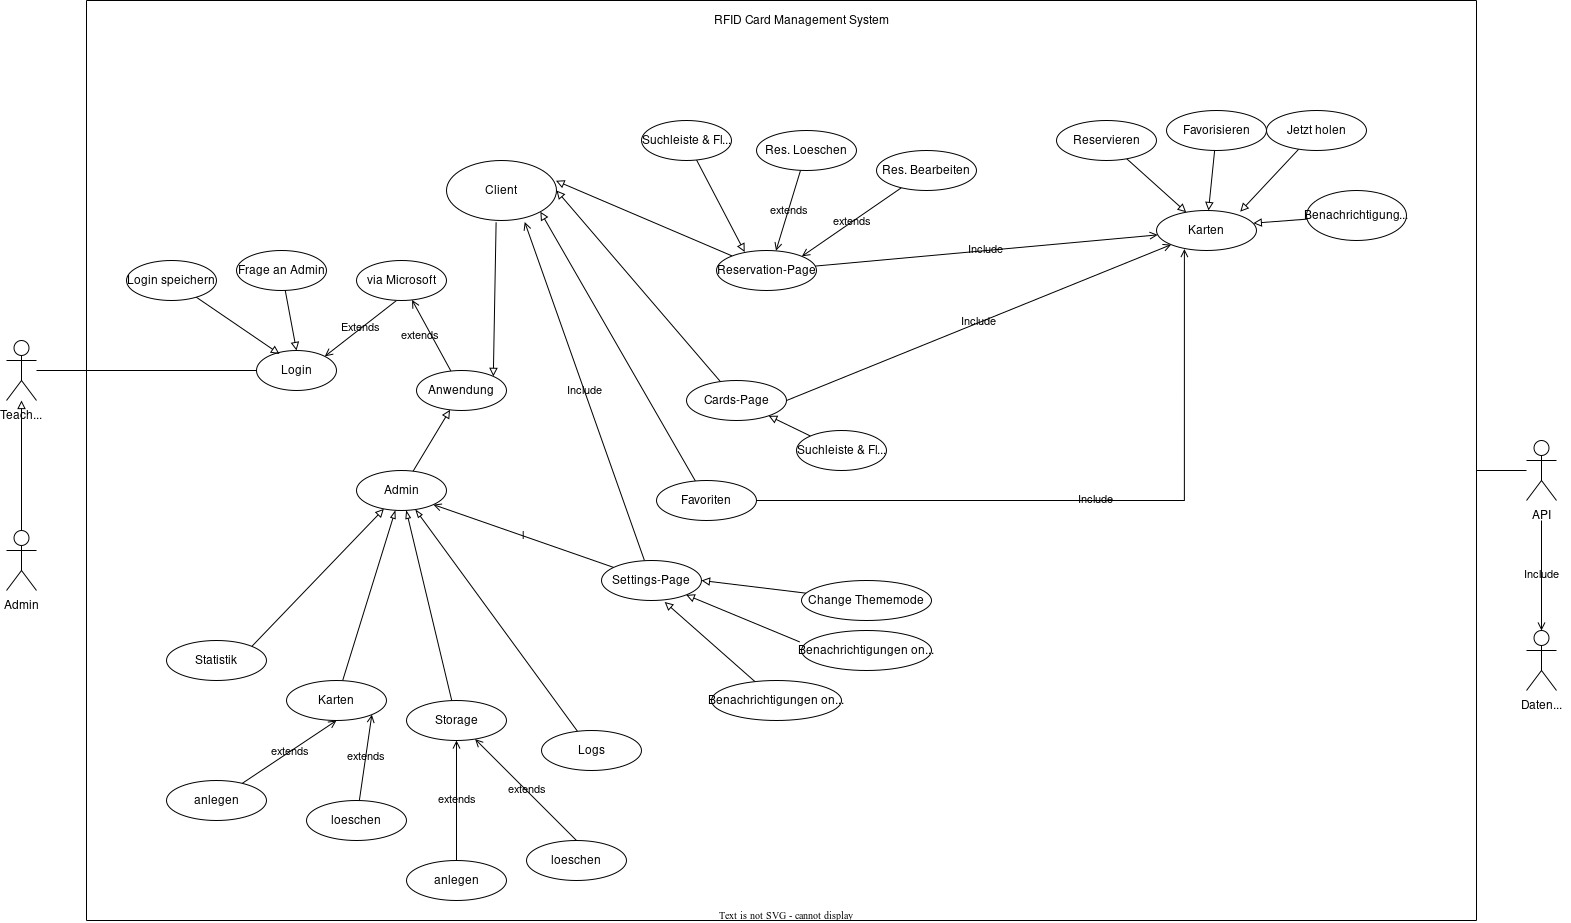
\includegraphics[width=0.9\textwidth]{FLUTTER/images/pflichtenheft/use_case.png}
\caption{Use Case}
\end{figure}
\newpage

\section{Mockups}

Hier folgen die Mockups:
\begin{figure}[h]
\centering
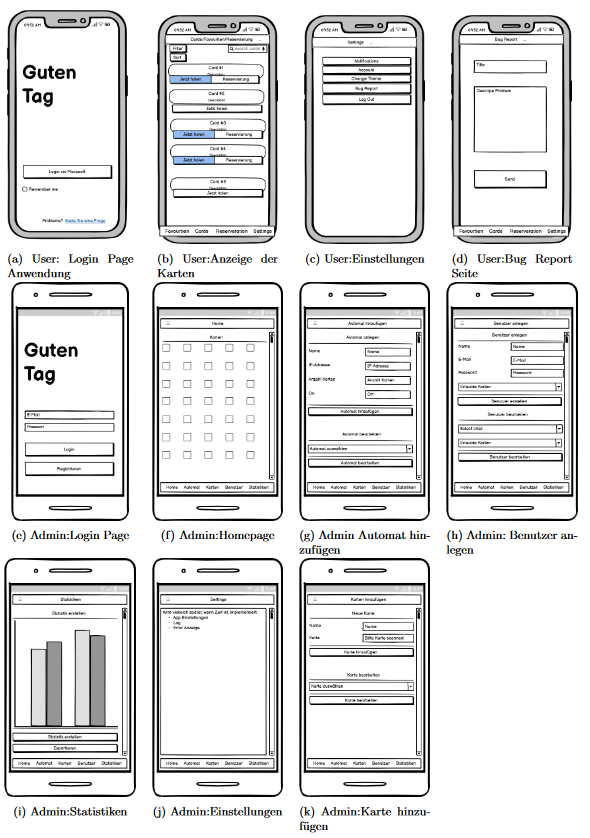
\includegraphics[width=0.7\textwidth]{FLUTTER/images/pflichtenheft/mockups.png}
\caption{Mockups}
\end{figure}

\newpage

\section{Kriterien}
\subsection{Fertigstellungszeitraum}
Sp\"atestens bis 31.3.2023

\subsection{Zentrale API}
Die Zentrale API (siehe \ref{sec-central-api}) erfüllt folgende Kriterien:
\begin{itemize}
    \item Anwendungsprogrammierer sollen über die API Benutzer, Karten, und Schließfächer anlegen, abrufen, ändern und löschen können
    \item Anwendungsprogrammierer sollen die Möglichkeit haben über die API Karten als reserviert und wieder zurückgegeben zu melden
    \item Anwendungsprogrammierer sollen Daten zur Statistischen Auswertung durch den Administrator abrufen können (Häufigkeiten von Reservierungen von Karten etc.)
    \item Anwendungsprogrammierer sollen Daten zu Informationszwecken für den Administrator abrufen können (API-Logs: Zugriffe von Clients, etc.)
    \item Die API soll als Softwarepaket in Form eines portablen Docker-Containers zur Verfügung stehen
    \item Die API unterscheidet zwischen Administrator und Benutzer
    \item Administratoraccounts sind vordefiniert und werden in der Datenbank gespeichert 
\end{itemize}

\subsection{API -- Raspberry Kommunikation}
Die Kommunikation zwischen Zentraler API und Raspberry (siehe \ref{api-raspi-communication}) erfüllt folgende Kriterien 
\begin{itemize}
    \item Anwendungsprogrammierer tauschen etwaige Daten mit der API über MQTT aus
    \item Anwendungsprogrammierer tauschen etwaige Daten mit dem Python Program aus, welche die Motoren des Tresor und den Karten Leser Steuert.
\end{itemize}

\subsection{Login/Registrierungsseite}
\begin{itemize}
  \item Der User soll sich mittels seinem Microsoft Account einloggen
  \item Der User soll die Moglichkeit haben seinen Login zu speichern (Remember me)
    \item Der User soll beim Login die Möglichekeit haben Fragen an den Admin zu stellen

\end{itemize}

\subsection{Client Anwendung / Login}
\begin{itemize}
    \item Die Client-Anwendung soll ein Reservierungssystem f\"ur die Karten bieten
    \subitem - Reservierungen sollen bearbeitbar/l\"oschbar sein
    \subitem - Reservierungen sollen eine Benachrichtigung bei einem bevorstehenden Termin versenden
    \item Die Client-Anwendung soll einen Shortcut bieten um Karten direkt zu holen (ohne Anmeldung am Terminal)
    \item Die Client-Anwendung soll die Möglichkeit bieten bestimmte Karte zu favorisieren 
    \item Die Client-Anwendung soll eine Benachrichtigung versenden falls eine markierte Karte wieder frei geworden ist.
    \item Die Client-Anwendung soll eine Einstellungsseite bieten (Benachrichtigungen, Thememode, usw.)
    \item Die Client-Anwendung soll ein System zum Chatten mit anderen Lehrern bieten falls eine Karte verwendet die sie benötigen
      \item Möglichkeit Nachrichten an den Admin zu senden (Feedback, Bug-report, Verbesserungen [...])
\end{itemize}

\subsection{Admin Anwendung / Login}
Die Anforderungen an die Admin App gestalten sich folgendermaßen:
\begin{itemize}
  \item Der Admin soll Karten anlegen / löschen / bearbeiten können.
  \item Der Admin soll Karten Tresore anlegen / löschen / bearbeiten können.
  \item Der Admin soll Benutzer anlegen / löschen / bearbeiten können.
  \item Der Admin soll sich Statistiken anzeigen lassen können.
  \item Der Admin soll sich Logs anzeigen lassen können.
\end{itemize}

\section{Teilbereiche}
\subsection{Zentrale API} \label{sec-central-api}
Die API ist der zentrale Knotenpunkt zum Austausch von Daten zwischen Client Anwendung (Flutter App) und den Card-Storage\footnote{Schließfach, in dem die RFID Karten aufbewahrt werden}s. Die API kommuniziert mit den Card-Storages mithilfe MQTT welche jeweils ein Topic zugewiesen bekommen und so Daten senden als auch empfangen können. Die API speichert etwaige Daten in einer Datenbank. Diese Daten können ausschließlich von der API verwaltet werden. Gehostet wird diese auf einem Zentralen Server sodass der Zugriff auf die ebenfalls zentralisierte Datenbank vereinfacht wird und alle Daten synchron und konsistent miteinanander sind.

\subsubsection{Hardware}
Docker-fähiger Server mit Netzwerkzugang und zwei offenen TCP-Ports für HTTP und MQTT.

\subsubsection{Sofware}
Die oben beschriebene API wird mithilfe der Programmiersprache Go umgesetzt. SQLite wird als relationale Datenbank eingesetzt. Der Card-Storage Controller wird ebenfalls in Go umgesetzt, wobei dieser mit dem Modul der Kollegen kommuniziert welches die Kommunikation zwischen dem Raspberry Pi und dem Mikrocontroller, welcher die Hardware regelt, erledigt.

\subsubsection{Zugriff als Client}
Die Kommunikation zwischen der API und den Clients findet im Rahmen des HTTP-Protkolls mithilfe der REST (Representaional State Transfer) Architektur statt. Die Clients senden HTTP-Kommandos um Daten zu Karten, Schließfächern bzw. Benutzern, lesen, erstellen, ändern sowie löschen zu können. Um zwischen einfachen Benutzern und Administratoren zu unterscheiden sendet der Administrator einen speziellen HTTP-Header welchen die API überprüft, um dem Administrator privilegierte Daten übermitteln zu können.   

% optional arg [] displayed in TOC 
\subsubsection[Zugriff als Card-Storage Controller]{Zugriff als Card-Storage Controller\protect\footnote{Mikroprozessor (Raspberry Pi) auf welchem die Software zur Verwaltung des Schlie"sfaches läuft}}
Die Card-Storage Einheiten kommunizieren mit der API mithilfe dem MQTT Protokoll. Das Controller Programm welches auf dem Raspberry (bzw. ein anderer Mikroprozessor) der Card-Storage läuft,
kommuniziert mit der API, um die Kommandos welche die API von der Client bzw. Admin Anwendung erhält, auszuführen. Da API und Card-Storage, Daten möglicherweise bidirektional austauschen müssen, wäre hier das klassische Client-Server Modell unpassend. Die API weist jedem Card-Storage ein Topic zu, über welches gemeinsam kommuniziert werden kann. 

\subsubsection{Datenbank}
Jegliche Daten, die speichernswert sind, werden in der zentralen Datenbank, welche ausschließlich über die oben erläuterte API zugänglich ist, abgelegt, um diese zu einem späteren Zeitpunkt entweder von einem Administrator, einem einfachen Benutzer des Systems, oder einem Card-Storage Controller wieder abzurufen.   

\subsubsection{Zusammenfassung}
Die API ist das Herzstück des Systems. Sowohl die Client- und Admin-Anwendung als auch die Card-Storage Einheiten kommunizieren damit. Die API ist, wenn man so will, der Übersetzer zwischen den beiden. Sie übersetzt einerseits die Kommandos der Client- und Admin-Anwendung in MQTT-Befehle welche dann vom Card-Storage Controller ausgewertet und an die Schaltung weitergegeben werden. Andererseits verwaltet die API auch den Zugriff zur Datenbank, in welcher alle Card-Storages, Benutzer sowie Karten hinterlegt sind. 

\subsection{Anwendung}
Als Grundlage zur administrativen als auch benutzerspezifischen Verwaltung, kommt eine Flutter App zur Anwendung. Wir haben uns für dieses Framework entschieden, da es auf verschiedenen Plattformen bzw. Betriebssystem mit einer Version der Software läuft (Native Framework). Um zu dem Admin-Login zu gelangen, wird ein eigener Login bei der Login-Seite benötigt. D.h Admin und User Anwendung teilen sich ab den Login auf.

\subsubsection{Login/Registrierungsseite}
Der Login dient dazu, um zu der Admin bzw. User Anmeldung hinzugelangen.
\paragraph{Funktionen}
\begin{itemize}
  \item Anmeldung eines Lehrers via Microsoft
  \item "Remember me" $\rightarrow$ Funktion
  \item Quick Login/Registrierung Möglichkeit am Terminal mittels Rfid Karte der Lehrer 
\end{itemize}
  
\subsubsection{Client Anwendung / Login}
\paragraph{Generelle Spezifikation}\mbox{}\\
Der User Login wird von den Lehrenden verwendet, um Karten zu beantragen, reservieren, anzufordern [...]. Weiters soll der Login am Display als auch im Web zur Verfügung gestellt, damit wirklich jeder Zugang zum Automaten hat. 

\paragraph{Software}
\begin{itemize}
  \item Die Startseite wird dazu verwendeten seine favorisierten Karten anzeigen zu lassen
  \item Es soll eine Seite mit allen Karten angezeigt werden, wobei man die angezeigten Karten, anhand verschiedener Kriterien filtern bzw. suchen kann
  \item Eine eigene Seite zum Reservierungssystem
  \item Quick Card Get Möglichkeit mittels Pop-Up am Display.
  \item Es soll eine Benachrichtigung versendet werden falls eine markierte bereits verwendete Karten wieder frei ist.
\item Die Client-Anwendung soll ein System zum Chatten mit anderen Lehrern bieten falls eine Karte verwendet wird die sie benötigen
  \item Möglichkeit Nachrichten an den Admin zu senden (Feedback, Bug-report, Verbesserungen [...])
\end{itemize}

\subsubsection{Admin Anwendung / Login}
\paragraph{Generelle Spezifikation}\mbox{}\\
Der Admin Login soll dazu verwendet werden können, direkt am Display am Automaten, administrative Aufgaben erledigen zu können. Diese Anwendung soll auch als Webseite und APP zur Verfügung stehen, um solche Einstellungen nicht direkt Vorort machen zu müssen. Die Admin App wird ebenfalls mit Flutter erstellt. Um die Admin App benutzen können, wird es bestimmte Benutzer geben die sich als Admin anmelden können.

\begin{itemize}
  \item In der soll der Administrator sich Statistiken zu allen Karten anzeigen lassen können. Das soll dazu dienen, das der Admin erkennen kann ob eine bestimmte Karte merfach benötigt wird.
  \item Weiters soll man in der App einen neuen Automaten hinzufügen können, dazu muss man einige Parameter angeben wie Name, IP-Adresse, Anzahl Karten, Ort. Danach werden diese in einer Datenbank im Hintergrund eingepflegt. Es besteht ebenfalls die Option, Automaten zu bearbeiten und zu löschen. 
  \item In der App sollen auch neue Karten hinzugefügt, gelöscht, bearbeitet werden können oder Karten getauscht werden, dazu wird, wenn das Fenster geöffnet wird am Automaten angezeigt, dass die Karten zum Lesegerät gehalten werden soll, damit die Karte im System gespeichert werden kann.
  \item Weiters soll sich der Admin Logs zu der Datenbank und API anzeigen lassen können. Das soll dazu dienen, wenn Fehler auftreten, diese leicht erkennen und beheben zu können.
\end{itemize}

\paragraph{Die App soll folgende Funktion bieten:}
\begin{itemize}
 \item Statistiken anzeigen,
 \item Neuen Automaten anlegen / löschen / bearbeiten 
 \item Neue Karten hinzufügen / löschen / bearbeiten
 \item Logs anzeigen
\end{itemize}

\subsubsection{Hardware} \label{hardware}
Da ein wir ein crossplattform Framework verwenden, haben wir die M\"oglichkeit mit wenig Arbeit unsere Produkt auf allen Ger\"aten anzubieten. Hier eine Auflistung auf welchen Ger\"aten die Hardware laufen muss
\begin{itemize}
  \item Android Geräte grö\"ser API 24
  \item Smartphones mit Betriebssystemen wie IOS,Android
  \item Geräte die einen Browser Bieten
\end{itemize}

\newpage

\subsection{API - Raspberry Kommunikation} \label{api-raspi-communication}
Das Programm, welches am Mikroprozessor läuft und einerseits die Kommandos, beispielsweise die Schließfachtür per App öffnen, interpretiert und ausführt aber auch andererseits Daten an die API, wenn diese danach fragt, beispielsweise die aktuelle Anzahl der vorhandenen Schlüsselkarten im Schließfach, zurücksendet. Das Card-Storage Controller Programm kommuniziert mittels MQTT mit der API. Dieses wird mithilfe der Programmiersprache Go implementiert. Jeder Card-Storage Controller bekommt ein MQTT-Topic zugewiesen, womit dieser mit dem Broker (Zentrale API) kommunizieren kann. Um, wie oben erwähnt, Funktionen bereitstellen zu können die Hardware beinhaltet, welche von den Mechatronikern enwtickelt wird, beispielsweise die aktuelle Anzahl der vorhandenen Schlüsselkarten im Schließfach, muss der Cardstorage-Controller auch mit dem Mikrocontroller kommunizieren, welcher eben diese Hardware über die Serielle Schnittstelle steuert. \textbf{Sobald ein Konzept seitens der Mechatroniker zur Verfügung steht, (und ob die oben als Beispiel genannten Funktionen überhaupt von den Mechatronikern implementiert werden) werden Einzelheiten weiter erläutert.}

\subsubsection{Raspberry}
Der Raspberry wird dazu verwendet die Daten von der API per MQTT zu erhalten (siehe \ref{api-raspi-communication}). Dieser wir ein Python Program laufen haben, diese dient dazu die Motgoren im Storage  zu steueren. Weiters werden die Daten vom NFC Reader an die API gesendet. Eine weitere Aufgabe des Raspberry ist, unsere App darzustellen. Weitere Information bei \ref{hardware} Hardware.

\subsubsection{Display}
Das Display wird dazu verwendet, die Admin und Client App darzustellen. Diese werden auf dem Raspberry im Browser laufen, und müssen etwas angepasst werden, da gewisse funktionalität der App im Browser nicht gewährleistet ist. Das Display wird per proprietärer Raspberry Schnittstelle angschlossen.

\subsubsection{NFC Reader}
Der NFC Reader wird dazu verwendet, User beim ersten mal per Chip zu authentifizieren. Dies wird dann in die Datenbank gespeichert. Eine weitere Aufgabe ist es, beim zurückgeben die Karten zu Scannen und bei dem jeweiligen User herauszulöschen. Damit ist gewährleistet, das die Karte auch von anderen Benutzer verwendet werden kann.

\section{Anwendungsbereiche / Zielgruppe}
\subsection{Benutzer}
Unser komplettes System ist für die Verwendung am Linzer Technikum gedacht. Diese wird dort von den Lehrern und Administratoren verwendet. Die Lehrer haben die Möglichkeit, sich Karten auszuborgen und zu reservieren. Administratoren können das komplette System verwalten. Administratoren sind fix vergebene Benutzer können sich bei der Client Anwendung nicht anmelden.

\subsection{Einsatz Ort}
Das System wird am Linzer Technikum eingesetzt. Dort werden im Gebäude mehrere Karten Tresore platziert. In jedem Karten Tresor befinden sich jeweils 10 Karten. Diese Karten Tresore werden nicht von uns gefertigt.